\section{Конструкторская часть}

В этом разделе будут представлены схемы реализуемых алгоритмов.

\subsection{Полный перебор}

На рисунке~\ref{fig:bruteforce} приведена схема алгоритма решения задачи коммивояжера полным перебором. 

\begin{figure}
	\centering
	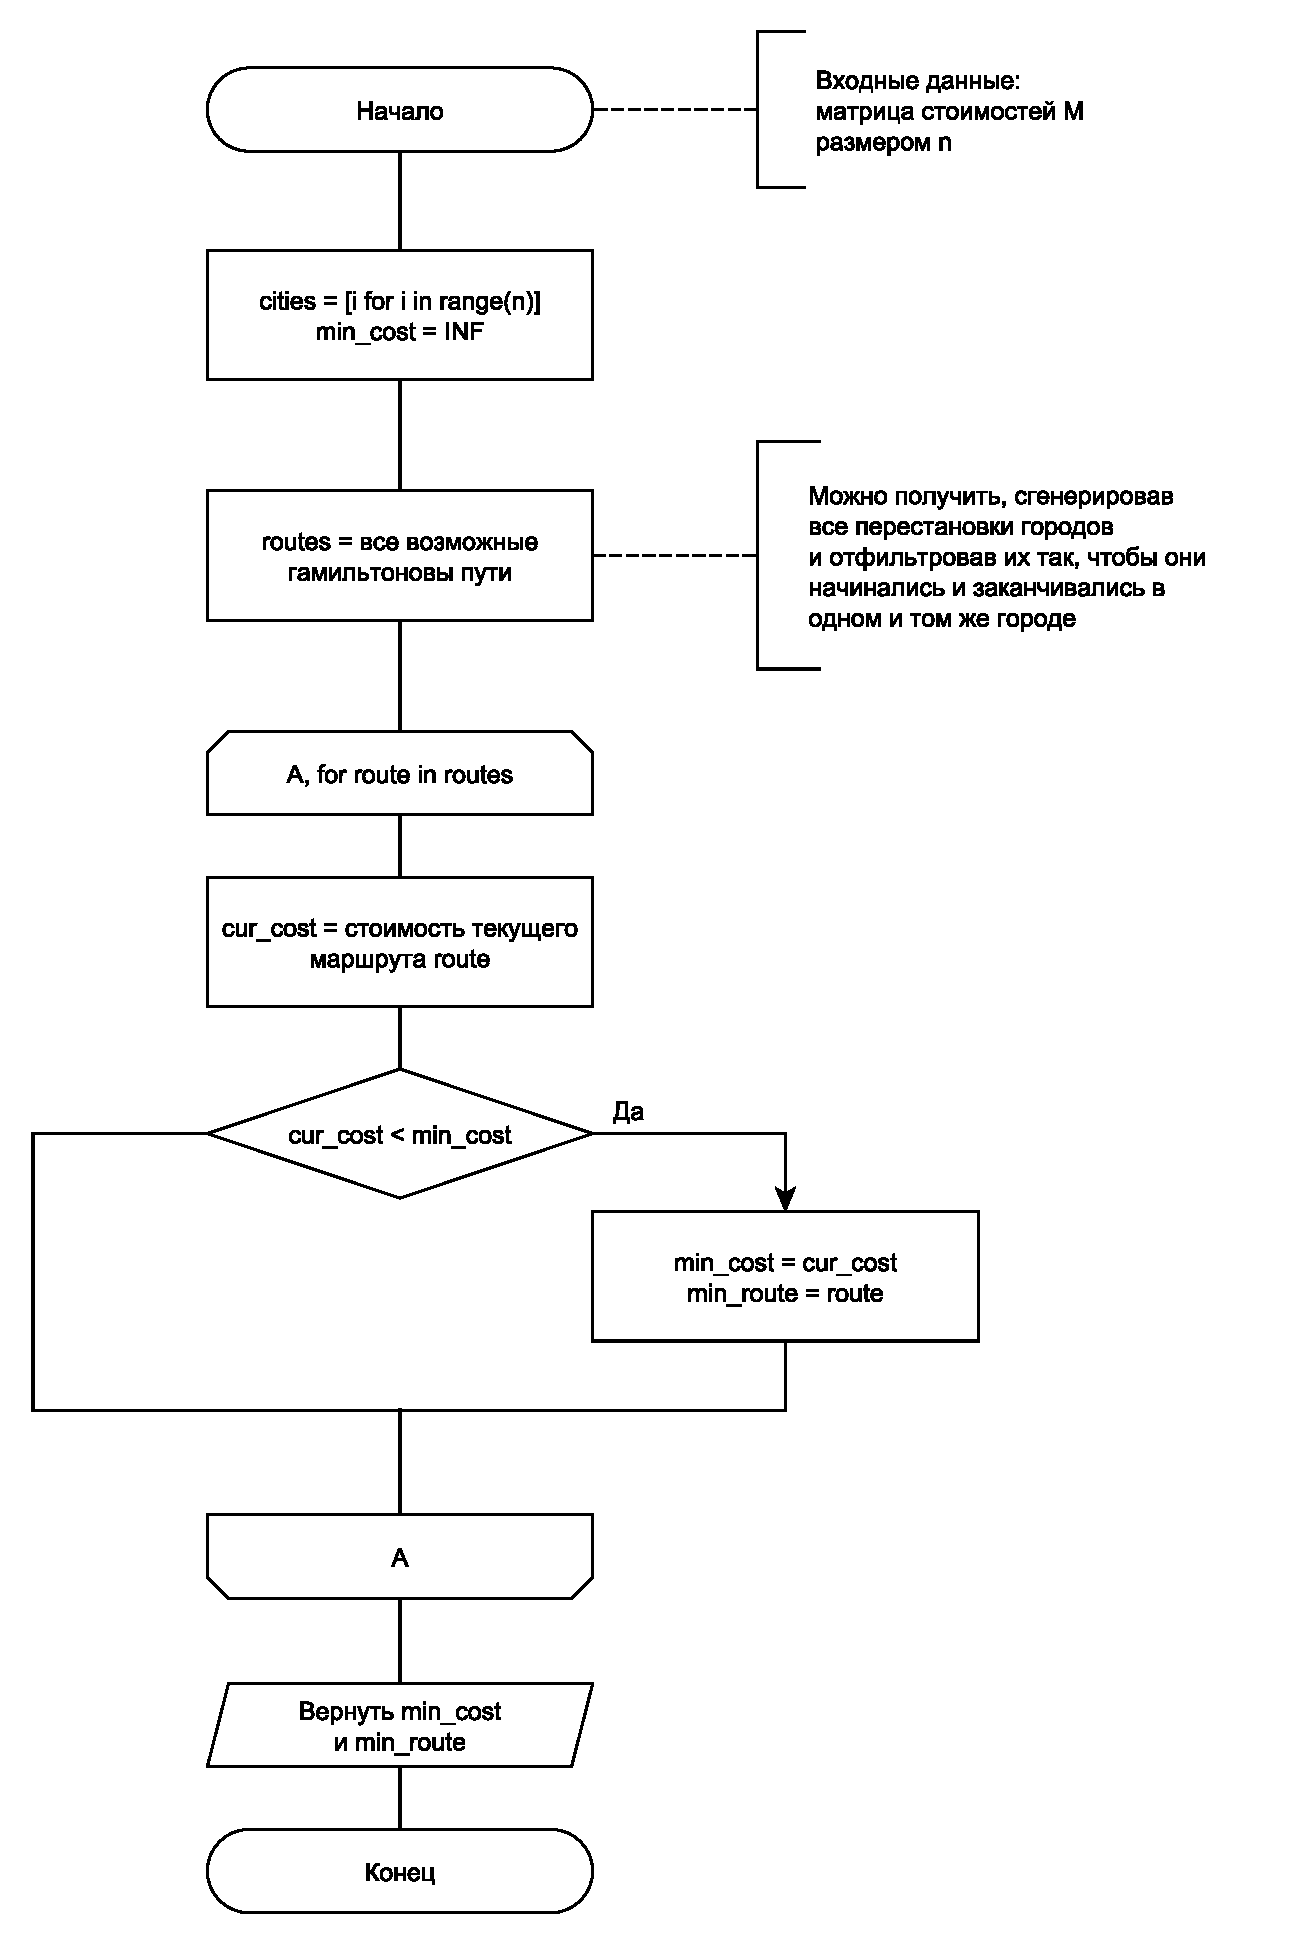
\includegraphics[width=0.65\linewidth]{images/bruteforce}
	\caption{Полный перебор}
	\label{fig:bruteforce}
\end{figure}

Преимущество алгоритма: оптимальный путь будет найден всегда.

Недостаток: скорость.

\subsection{Муравьиный алогритм}

На рисунке~\ref{fig:ant} приведена схема алгоритма решения задачи коммивояжера муравьиным алгоритмом. 

\begin{figure}
	\centering
	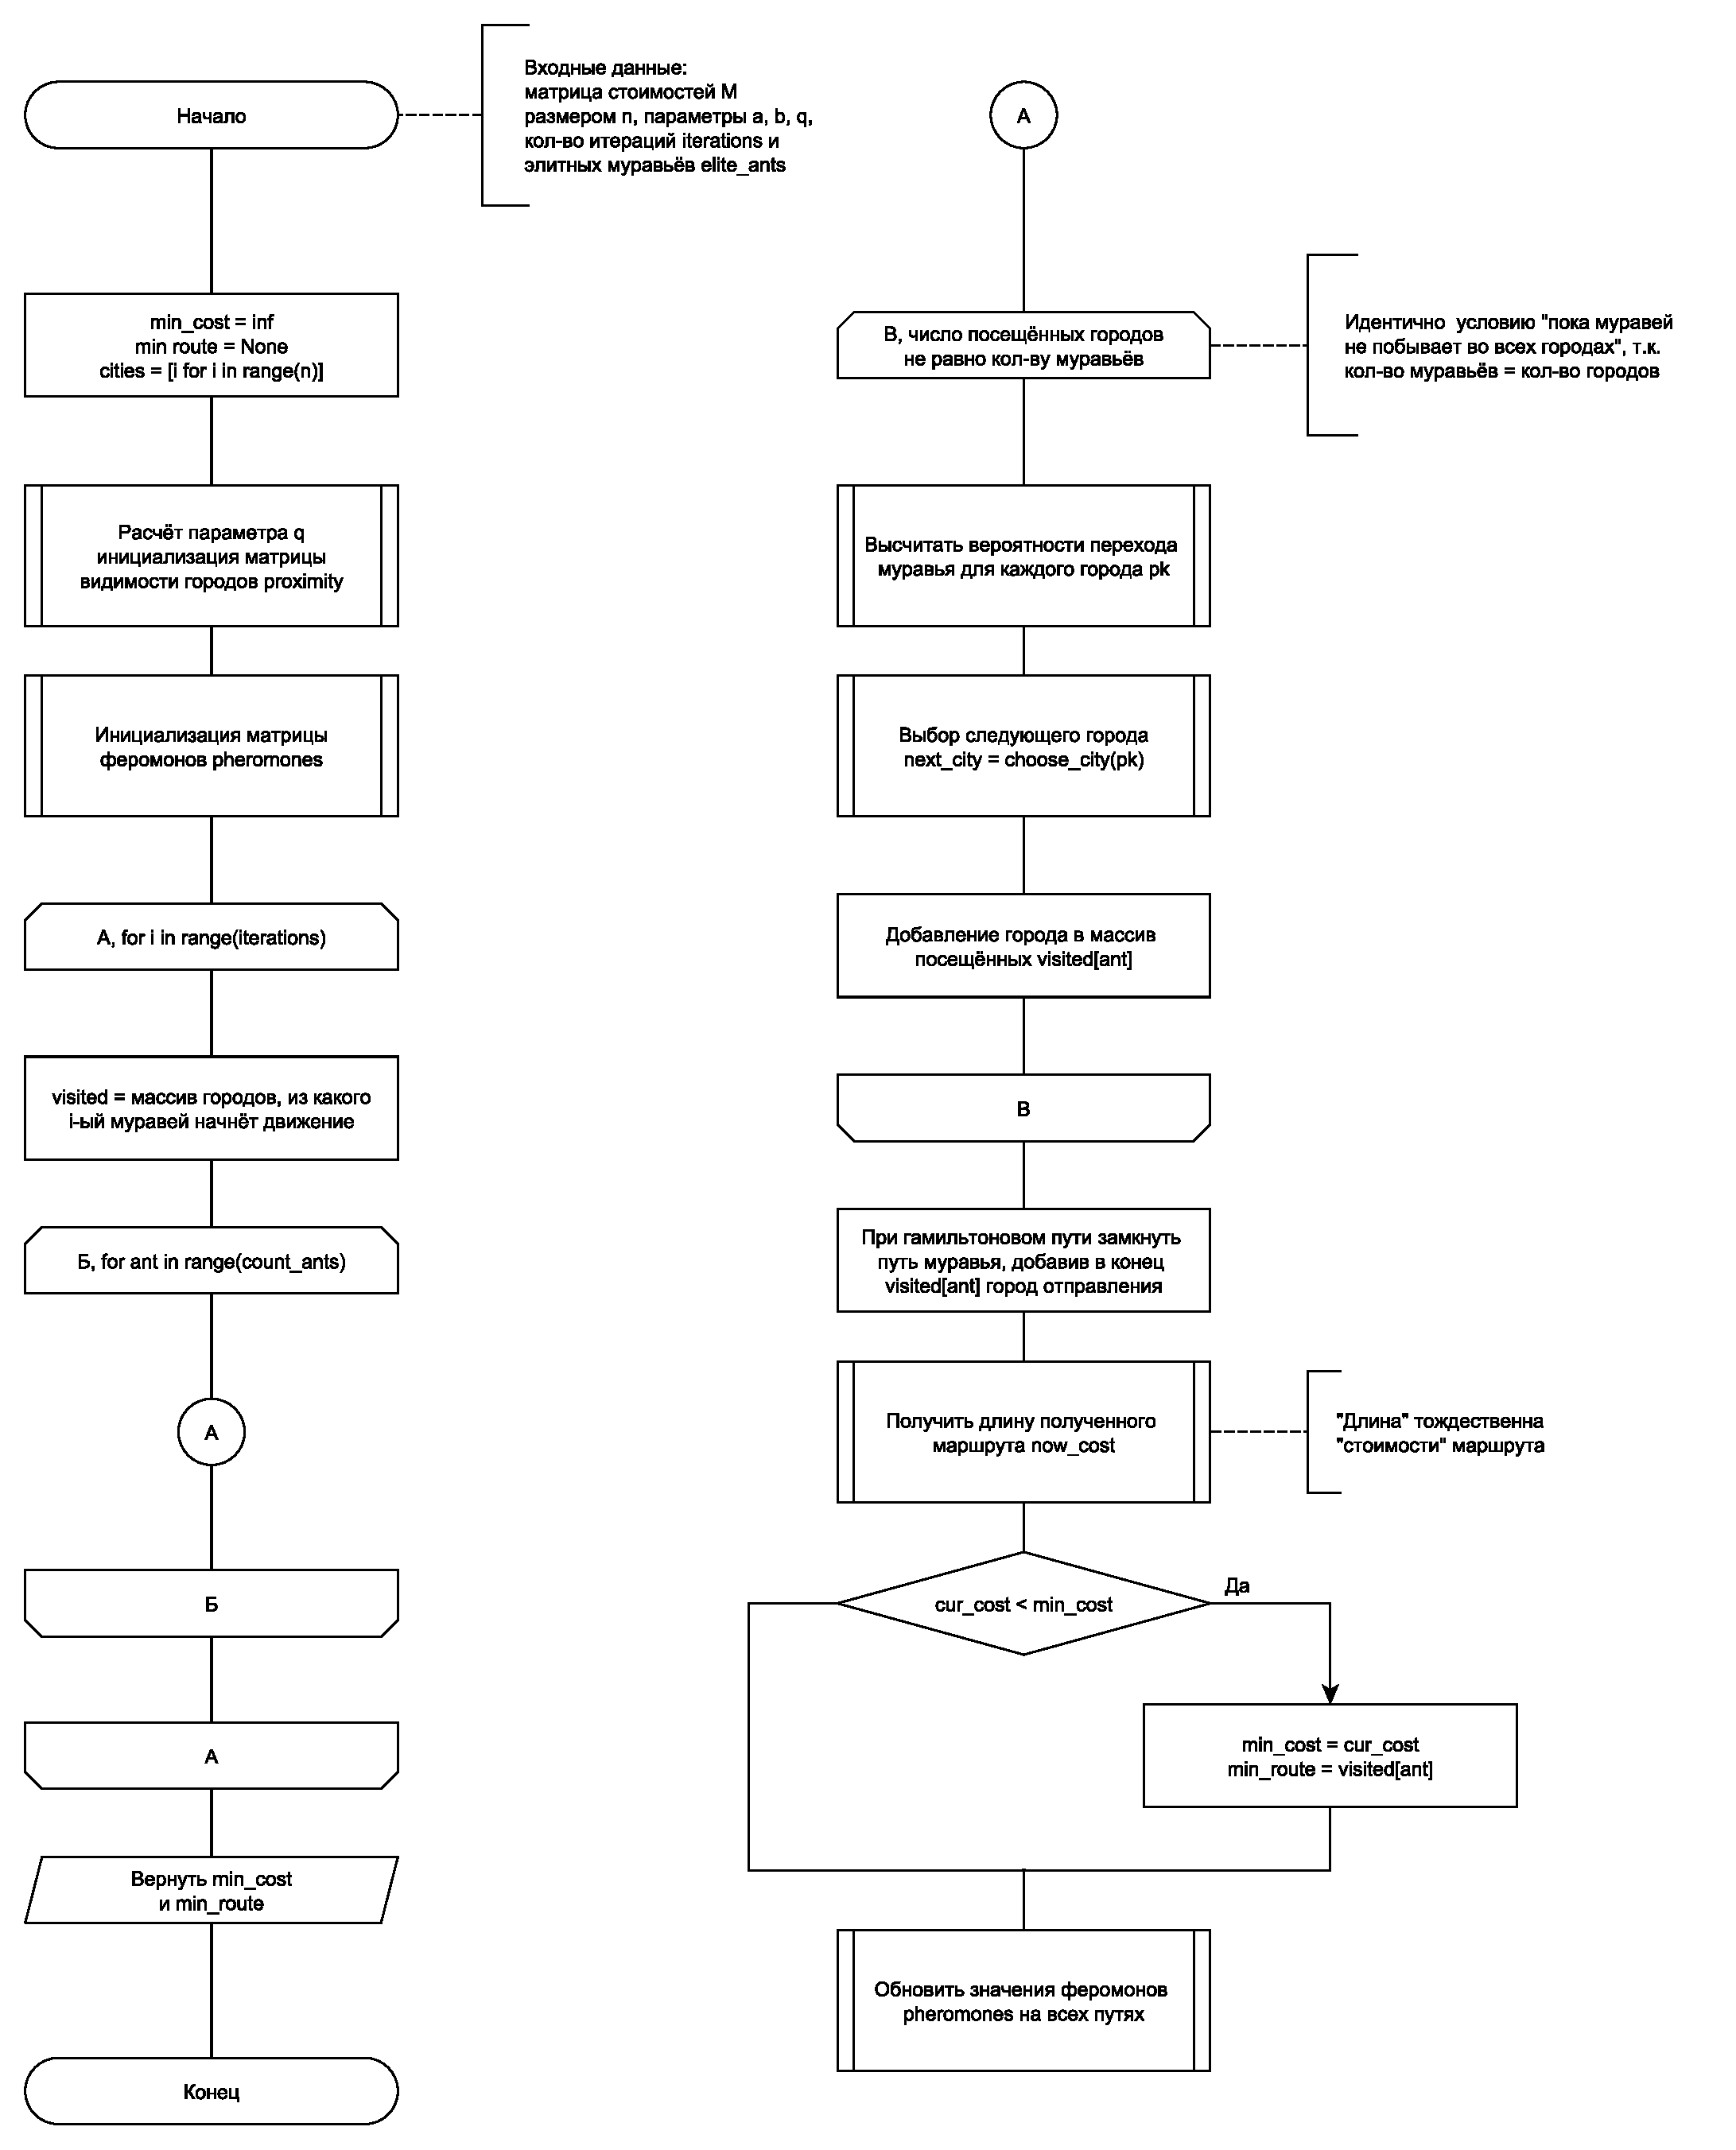
\includegraphics[width=1.0\linewidth]{images/ant}
	\caption{Муравьиный алгоритм}
	\label{fig:ant}
\end{figure}

На рисунке~\ref{fig:probabilities} приведена схема алгоритма вычисления вероятностных переходов.

\begin{figure}
	\centering
	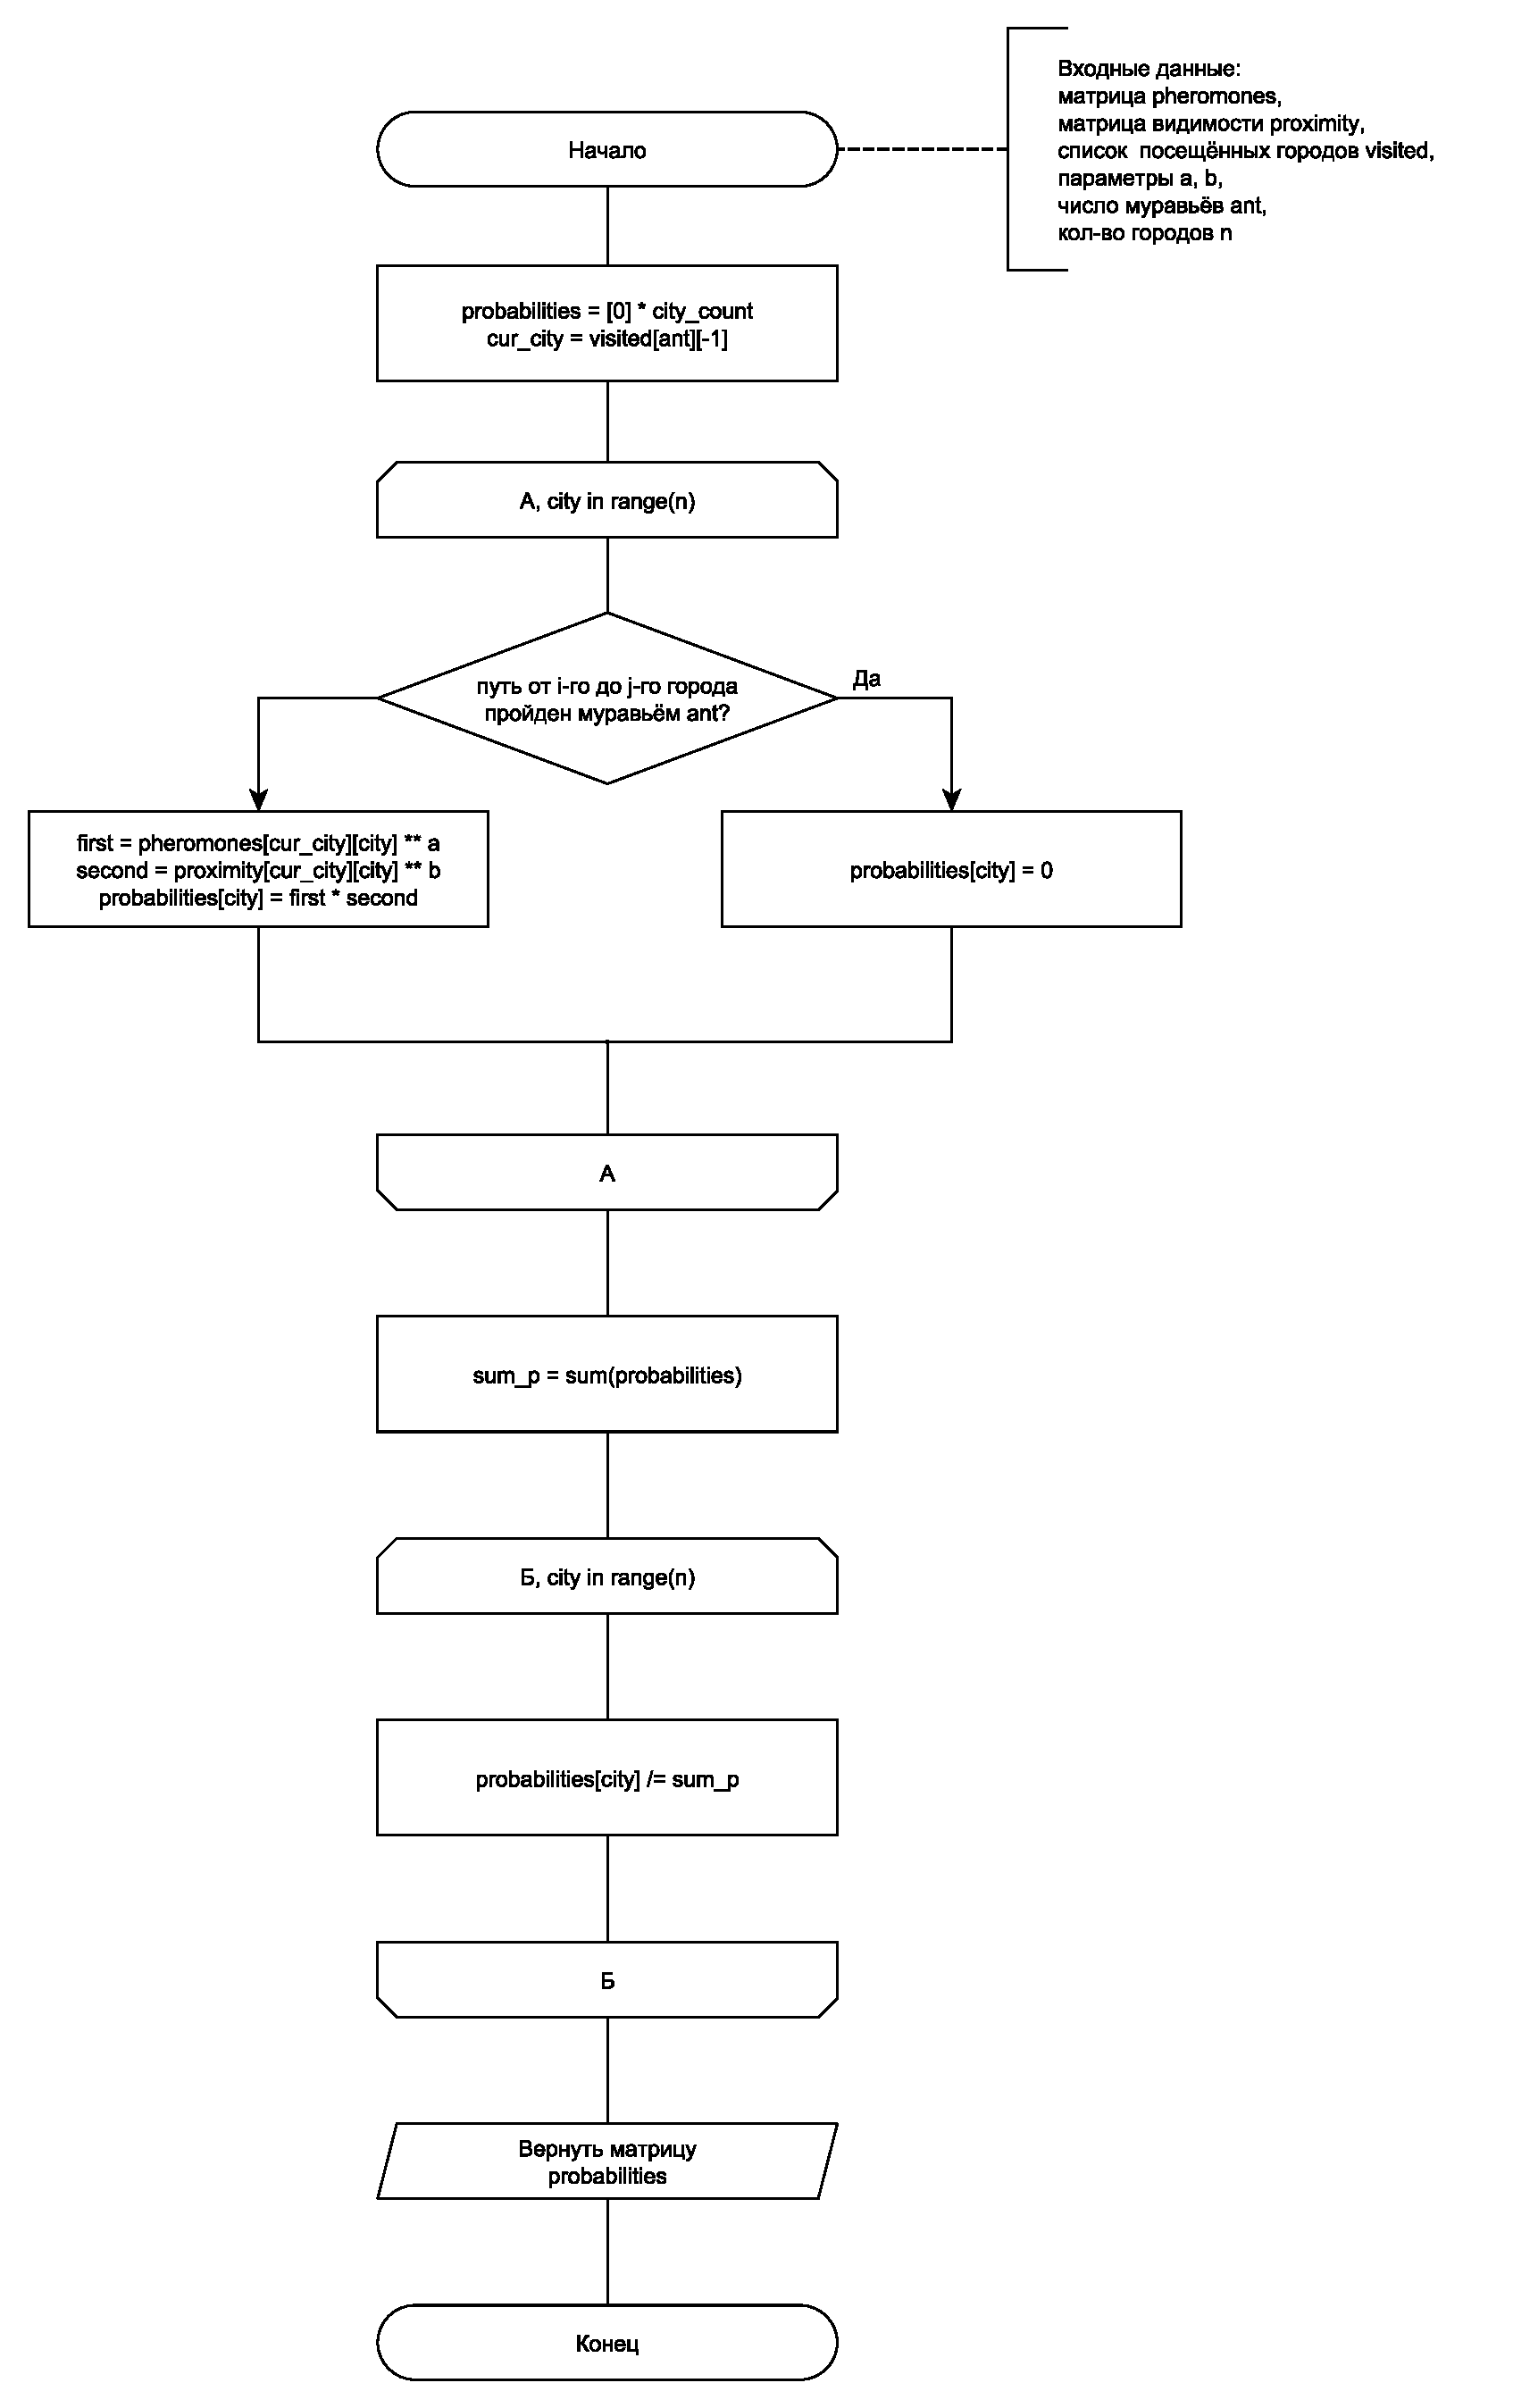
\includegraphics[width=0.85\linewidth]{images/probabilities}
	\caption{Вычисление вероятностных переходов}
	\label{fig:probabilities}
\end{figure}

На рисунке~\ref{fig:pheromone} приведена схема алгоритма обновления кол-ва феромонов на путях.

\begin{figure}
	\centering
	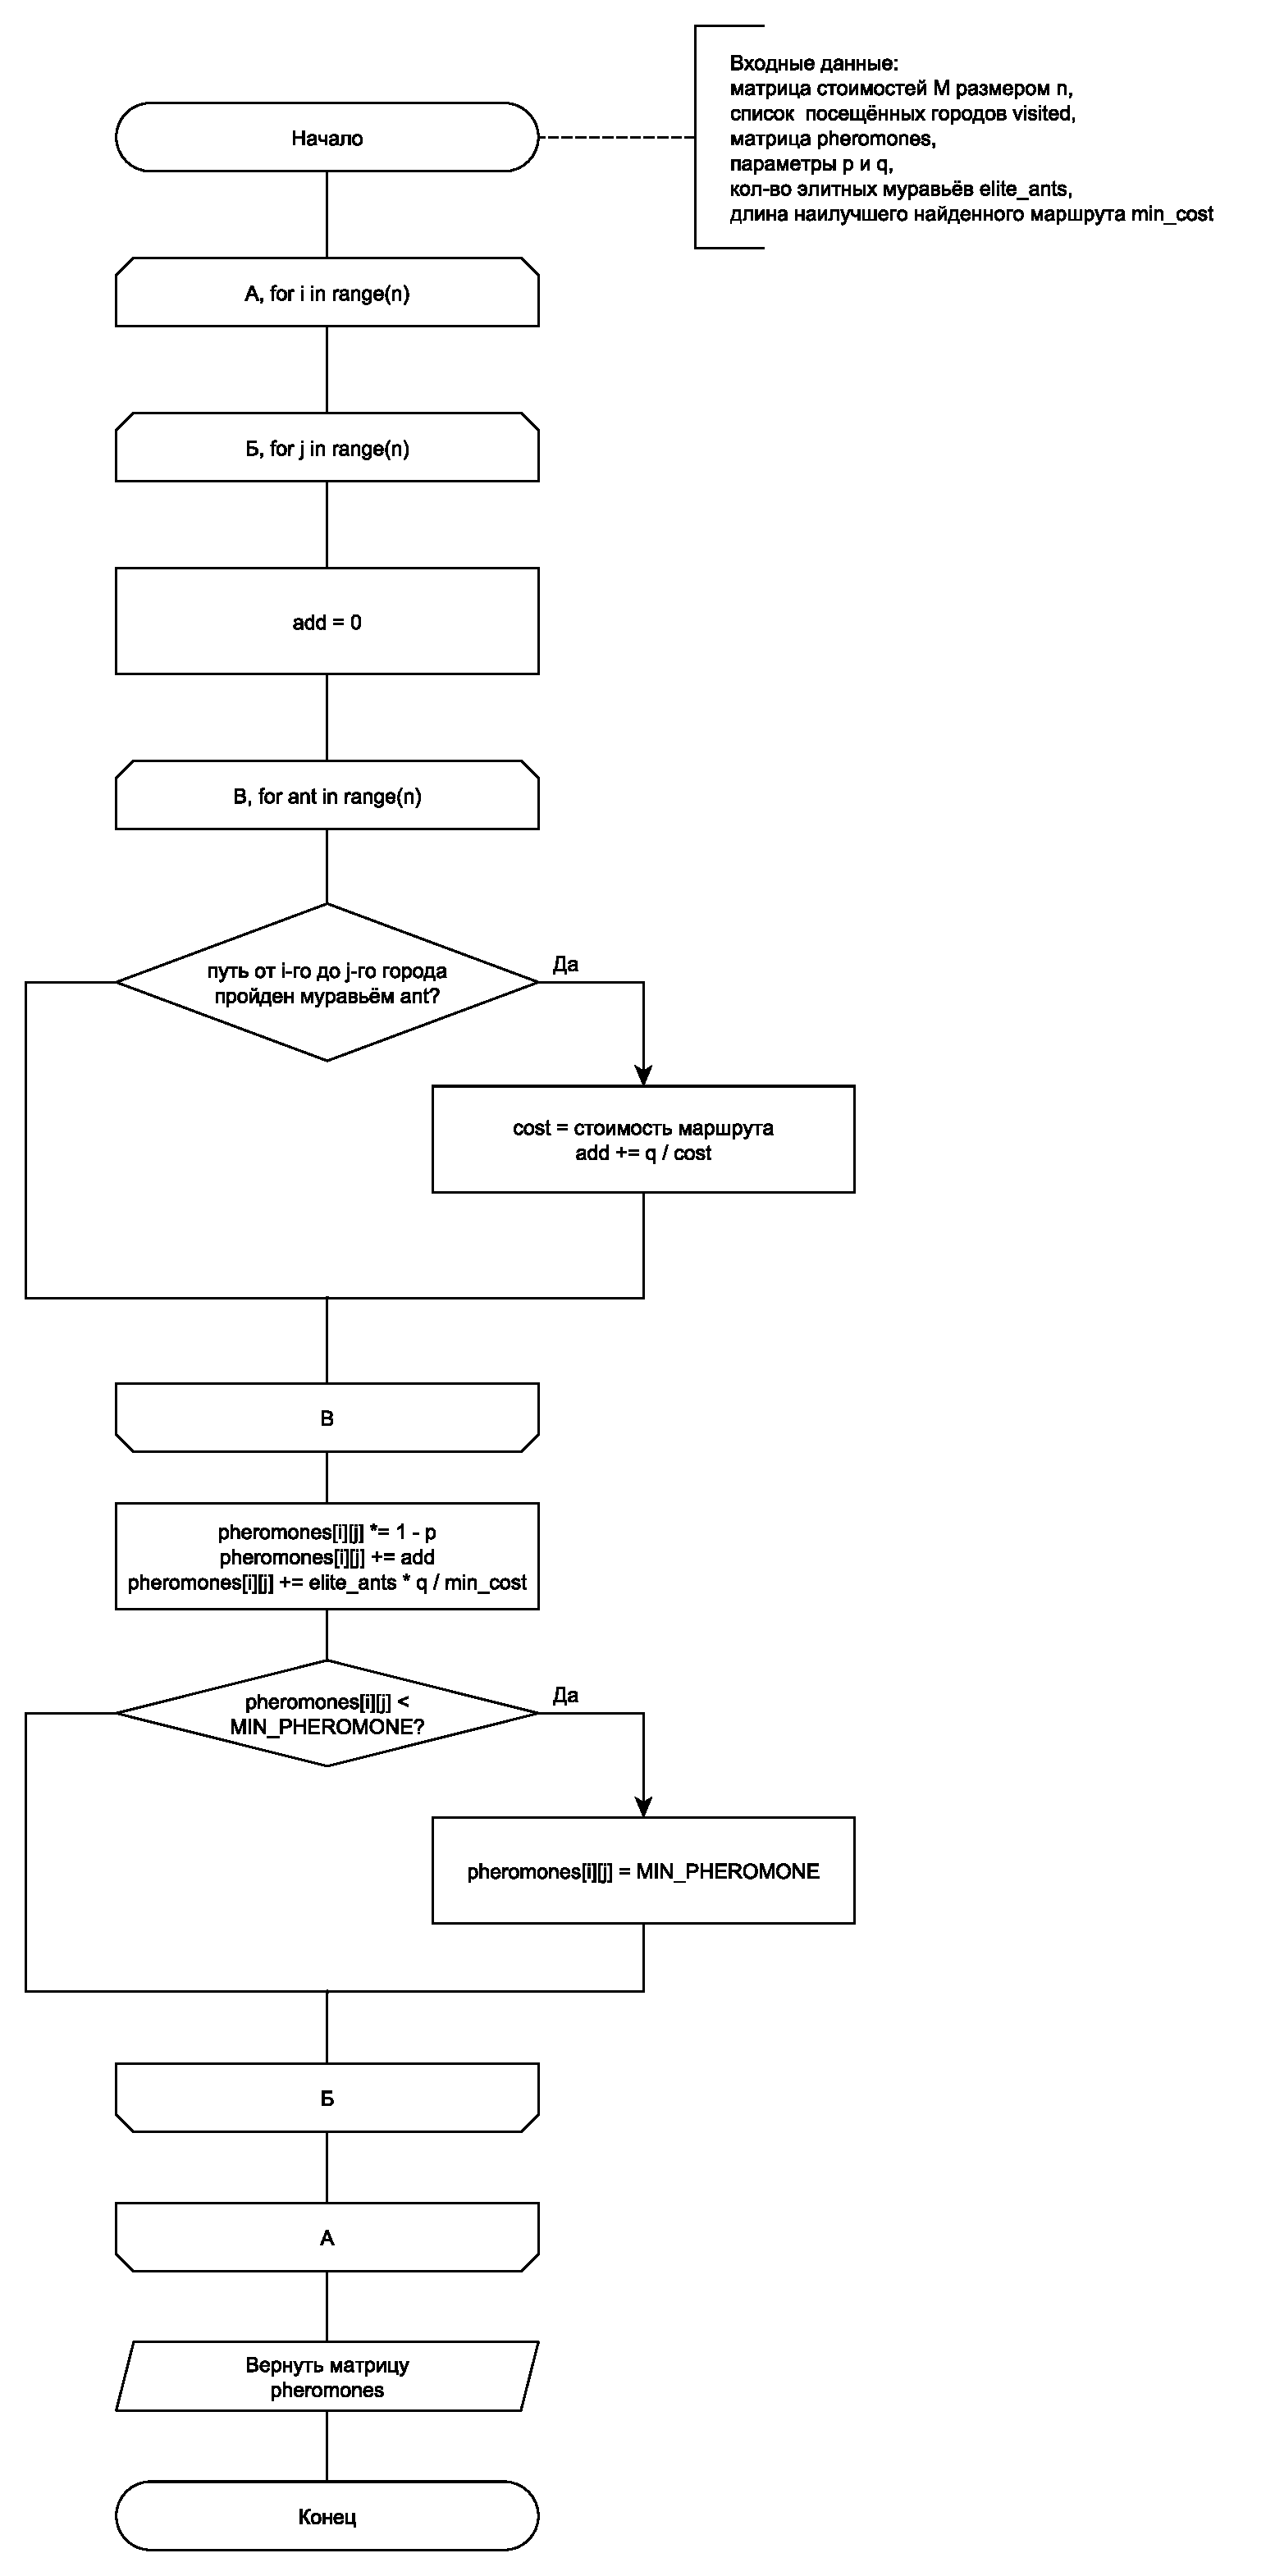
\includegraphics[width=0.65\linewidth]{images/pheromone}
	\caption{Обновление феромона}
	\label{fig:pheromone}
\end{figure}

Обратите внимание: по варианту необходимо рассмотреть муравьиный алгоритм с элитными особями.
Элитный муравей усиливает ребра наилучшего маршрута, найденного с начала работы алгоритма \cite{штовба2003муравьиные}.
Именно поэтому к значению $pheromones[i][j]$ добавляется значение $\dfrac{elite\_ants \cdot q}{ min\_cost}$.
В алгоритме без элитных муравьёв этого слагаемого нет.

Остальные схемы подпрограмм, указанные на рисунке~\ref{fig:ant} не приведены, т.к. они зависят от конкретной реализации.
Подпрограммы рисунках~\ref{fig:probabilities} и~\ref{fig:pheromone}, в свою очередь, от реализации к реализации не меняются (за исключением модификаций метода, таких как добавление элитных муравьёв).

Преимущество метода: скорость.

Недостаток: для нахождения оптимального пути требуется увеличение итераций и подбор параметров опытным путём.